\chapter{Sampling and stratification\label{samp}}

Sampling consists in predicting the characteristics of a set from one part (a sample) of this set. Typically, we want to estimate the volume of wood in a forest, but it is impossible to measure the volume of all the trees one by one. We therefore measure the volume of a sample of trees in the forest, then extrapolate to obtain an estimate for all the trees in the entire forest \citep[p.252]{ctft89}. As volume is measured only in a sample of trees, the estimated total volume we obtain suffers from a \emph{sampling error}\footnote{The terms in italics are those used in sampling theory; a definition of these terms may be found, for example, in appendix 2 of \citet{bellefontaine01}.}.
Sampling in the strict sense consists in:
\begin{enumerate}
\item selecting appropriate trees for the measured set (we tend to speak of a \emph{sampling plan}),
\item selecting a method used to calculate total volume from the measurements (we tend to speak of an \emph{estimator}),
\end{enumerate}
in such a manner to minimize the sampling error.

In conventional sampling theory, the volumes of $N$ trees in the stand are fixed data: the only source of variation in the estimations is the sampling, such that exhaustive sampling would always give the same estimation. Here in this guide we will adopt the so-called super-population approach that was developed in the 1970s \citep{cochran77}. This consists in considering that the volumes of the $N$ trees that make up the stand are random variables, such that the observed stand is only one among others drawn from a super-population. This approach means that we can do away with certain approximations and draw up an optimal sampling plan (something that is often impossible in the conventional approach). It does, however, have the disadvantage of leading to incorrect solutions if the super-population model adopted does not comply with reality.

The sampling method depends on the goal. Therefore, in principle, the question must first be asked as to the purpose of the volume or biomass tables we are seeking to construct. Are they to serve to predict the characteristics of a particular tree that has known entry variables? Are they to serve to predict the characteristics of an average tree from data on entry variables? Are they to serve to predict the total volume of the stand that yielded the trees used to construct the tables, or the total volume of another stand? In both these latter cases, are the tables' entry variables measured in all the trees of the stand, or again on a sample of trees? Etc. We can therefore construct a chain that runs from the studied stand to the variable we are looking to predict (Figure \ref{cha}).

\begin{figure}[htb]
\begin{center}\setlength{\unitlength}{1cm}
\begin{picture}(15,4.5)(0,-1.2)
\put(0,0){\shortstack{Stand\\ studied}}
\put(2.2,0.5){\vector(1,0){2.2}}\put(2.6,0.6){\scriptsize sampling}
\put(2.9,0.2){\scriptsize plan}
\put(4.5,0){\shortstack{Trees\\ measured}}
\put(6,0.5){\vector(1,0){2.2}}\put(6.6,0.6){\scriptsize
model}\put(6.4,0.2){\scriptsize construction}
\put(8.4,0.3){Model}\put(9.5,0.5){\vector(1,1){2.2}}
\put(9.5,0.5){\vector(3,1){2.2}}\put(9.5,0.5){\vector(3,-1){2.2}}
\put(9.5,0.5){\vector(1,-1){2.2}}\put(9.5,2){\scriptsize
prediction}\put(9.5,-1.5){\scriptsize extrapolation}
\put(11.8,2.7){\shortstack{Volume of an\\ individual tree}}
\put(11.8,1.23333){\shortstack{Mean tree\\ volume}}
\put(11.8,-0.23333){\shortstack{Volume of the\\ studied stand}}
\put(11.8,-1.7){\shortstack{Volume of\\ another stand}}
\end{picture}
\end{center}
\caption[Chain running from the studied stand to the variables we are looking to predict]{Chain running from the studied stand to the variables we are looking to predict. \label{cha}}
\end{figure}

By following this chain backward, it can be seen that the precision of the predicted variable depends on the precision of the tables' parameters, which itself depends on the sampling plan (number and selection of trees measured) and the variability within the studied stand \citep{cunia87c}. We can therefore set a target for the precision of our predictions which, by a retroactive effect for a given table and a given sampling type, determines the minimum number of trees to be measured. We can also apply an optimization procedure to determine, for a given target precision and a given table, the sampling method that minimizes measurement time or cost \citep{cunia87,cunia87d}. In certain cases the cost of the measurements is the limiting factor. This in particular is the case for biomass measurements of root systems. Here in this case we are not looking so much to reach a given target precision in our prediction but to remain within reasonable cost limits. We can therefore, for a given measurement cost and a given type of table, determine the sampling plan that maximizes the precision of our predictions.

This reasoning, which is often too complex to be followed in a rigorous manner, should be applied on a case-by-case basis as it depends (\textit{i}) on what we are looking to predict, (\textit{ii}) on the type of tables used and (\textit{iii}) on the type of sampling adopted. The fact that we are using a table is in itself a constraint on the sampling method: the total volume of a stand can be estimated from the volume of a sample of trees, without using volume tables. By using volume tables to estimate the total volume of a stand, we are already restricting ourselves to one type of total volume \textit{estimator}.

What is more, the reasoning used to determine the sampling plan that complies with the target precision for our predictions assumes that we know the relation between the precision of our predictions and the precision of the parameters used to construct the tables, and the relation between the precision of the parameters used to construct the tables and sample size, etc. In certain simple cases these relations are explicitly known. But in most cases, as soon as the tables take a more complex form, these relations are not explicit. In this case, the above reasoning is no longer tractable.

This reasoning is delivered a knock-out blow when we realize that: (\textit{i}) volume/biomass tables generally have multiple purposes or unspecified purposes and (\textit{ii}) the form of these tables is generally unknown in advance. This is due to the simple fact that in most cases we wish to use these tables for different ends: to estimate the volume of a particular tree, an average tree, an entire stand, etc. Constructing the tables is ultimately an end in itself, without any reference to a quantity we wish to predict. Also, the form of the table is most often selected based on the results of an exploratory data analysis, and is therefore not known in advance. Obviously, some relationships such as the power function or second-order polynomials often recur, but no rule can be established \textit{a priori}. It is therefore illusory to look to optimize a sampling plan.

Ultimately, the sampling used to construct volume/biomass tables is generally based on empirical considerations relating to the sampling plan. The choice of the \textit{estimator}, which in fact determines which tables are chosen is made \textit{a posteriori}, depending on the data collected, and independently of the sampling plan.

\section{Sampling for a simple linear regression\label{simple}}

Let us begin with a simple example that clearly illustrates the notions developed above. Let us assume that the trees in a given stand are described by their dbh $D$, their height $H$ and their volume $V$. We use volume tables that predict volume $V$ from the variable $D^2H$. The super-population model we adopt to describe the stand assumes that the relation between $V$ and $D^2H$ is linear, with white noise $\varepsilon$ of variance $\sigma^2$:
\begin{equation}
V=\alpha+\beta\,D^2H+\varepsilon\label{MLex}
\end{equation}
where $\varepsilon$ follows a normal distribution of zero expectation and standard deviation $\sigma$. Let us also assume that the quantity $D^2H$ follows a normal distribution with a mean of $\mu$ and a standard deviation of $\tau$. White noise $\varepsilon$ incorporates all the factors that cause two trees of the same dbh and the same height not to have necessarily the same volume. Parameters
$\alpha$ and $\beta$ are unknown. To estimate them, we will measure 
$n$ trees; and will thus obtain a sample of $n$ doublets
$(D_1^2H_1,\,V_1)$, \ldots, $(D_n^2H_n,\,V_n)$, then construct the following linear regression:
\begin{equation}
V_i=a+b\,D_i^2H_i+\varepsilon_i\label{reg}
\end{equation}
In sampling theory jargon, the entry variables for the volume/biomass tables (diameter, height\ldots) are called \emph{auxiliary} variables. It is important to distinguish these tree-related variables from those such as age which are stand-related. These latter variables are considered as parameters \citep[p.106]{parde88}. Also, the sampling \emph{unit} is the tree. Let us now see how to draw up a sampling plan on the basis of the goal set.

\subsection{Predicting the volume of a particular tree}

Let us assume that the goal is to predict the volume of a tree in a stand of dbh $D^*$ and height $H^*$. Its predicted volume is of course:
\[
V^*=a+b\,D^{*2}H^*
\]
The super-population model stipulates that because of white noise 
$\varepsilon$, two trees selected at random and with the same dbh $D$ and the same height $H$ do not necessarily have the same volume. This means we are faced with intrinsic variability when we measure a particular tree, equal to $\sigma^2$. When attempting to predict volumes, this intrinsic variability is supplemented by the variability due to the imprecision of the $\alpha$ and $\beta$ parameter estimations. We will return to these notions later (in chapter \ref{util}). Thus, for a linear regression, the semi-amplitude of the confidence interval at the threshold $\alpha$ (typically 5\,\%) of $V^*$ is equal to \citep[p.374]{saporta90}:
\[
t_{n-2}\;\hat{\sigma}\,\sqrt{1+\frac{1}{n}+
\frac{(D^{*2}H^*-\overline{D^2H}_e)^2}{\sum_{i=1}^n(D_i^2H_i
-\overline{D^2H}_e)^2}}
\]
where $t_{n-2}$ is the quantile $1-\alpha/2$ of a Student's distribution with 
$n-2$ degrees of freedom, $\overline{D^2H}_e$ is the empirical mean of the $D^2H$ values measured in the sample:
\[
\overline{D^2H}_e=\frac{1}{n}\sum_{i=1}^nD_i^2H_i
\]
and $\hat{\sigma}$ is an estimate of the standard deviation of the residuals:
\[
\hat{\sigma}^2=\frac{1}{n-2}\sum_{i=1}^n[V_i-(a+b\,D_i^2H_i)]^2
\]
The lowest value of this semi-amplitude (when $n\rightarrow\infty$) is $\decimal{1}{96}\,\sigma$. We will now set our precision target for the estimation as a deviation of $E\,\%$
from this incompressible minimum, i.e. in an approximate manner we are looking for sample size $n$
such that:
\begin{equation}
1+E\approx\sqrt{1+\frac{1}{n}+
\frac{(D^{*2}H^*-\overline{D^2H}_e)^2}{\sum_{i=1}^n(D_i^2H_i
-\overline{D^2H}_e)^2}}\label{E1}
\end{equation}

\subsubsection{Random sampling}

Let us first examine the case where we do not look to optimize the sampling plan, for example by selecting sample trees at random. The empirical mean of $D^2H$ in the sample is therefore an estimation of $\mu$, while the empirical variance of $D^2H$ in the sample is an estimation of $\tau^2$. Thus:
\[
(1+E)^2-1\approx\frac{1}{n}\left[
1+\frac{(D^{*2}H^*-\mu)^2}{\tau^2}\right]
\]
By way of a numerical example, let us take $\mu=5$ m$^3$ as the mean value of $D^2H$ in the entire stand and $\tau=1$ m$^3$
as its standard deviation. If we want to predict the volume of a tree that has a $D^2H$ of 2 m$^3$ with a precision deviation of $E=5\,\%$, we will have to measure approximately $n=98$ trees.
We can see here that the expression of $n$ in relation to $D^{*2}H^*$
is symmetrical around $\mu$ and passes through a minimum for $D^{*2}H^*=\mu$. As $\mu-2=3$ m$^3$ and $\mu+3=8$ m$^3$, we will also need $n=98$ trees to predict the volume of a tree whose $D^2H$ is 8 m$^3$ with a precision deviation of 5\,\%. The $n=98$ sample size may also be interpreted as that which ensures a precision deviation of at most 5\,\% (at $\alpha=5\,\%$) for all predictions in the 2--8 m$^3$ range.

\subsubsection{Optimized sampling}

Let us now examine the case where we are looking to optimize the sampling plan in relation to the value of $D^{*2}H^*$. Equation (\ref{E1}) shows that precision deviation $E$ is smallest when $\overline{D^2H}_e=D^{*2}H^*$. It is therefore advantageous to select sample trees in such a manner that their empirical mean $D^2H$ value is $D^{*2}H^*$. In practice, as the empirical mean of the sample's $D^2H$ values will never be exactly $D^{*2}H^*$, it is advantageous to maximize the denominator $\sum_i(D_i^2H_i-\overline{D^2H}_e)^2$, i.e. to maximize the empirical variance of the sample's $D^2H$ values. Ultimately, the sampling plan that maximizes the precision of the volume prediction of trees with $D^2H$ values of $D^{*2}H^*$ consists in selecting $n/2$ trees with $D^2H$ values of $D^{*2}H^*-\Delta$ and $n/2$ trees with $D^2H$ values of $D^{*2}H^*+\Delta$, with $\Delta$ being as large as possible (Figure \ref{plan}).
\begin{figure}[htb]
\begin{center}
\setlength{\unitlength}{1cm}%
\begin{picture}(14,4.5)(0,-1)
\put(0,0){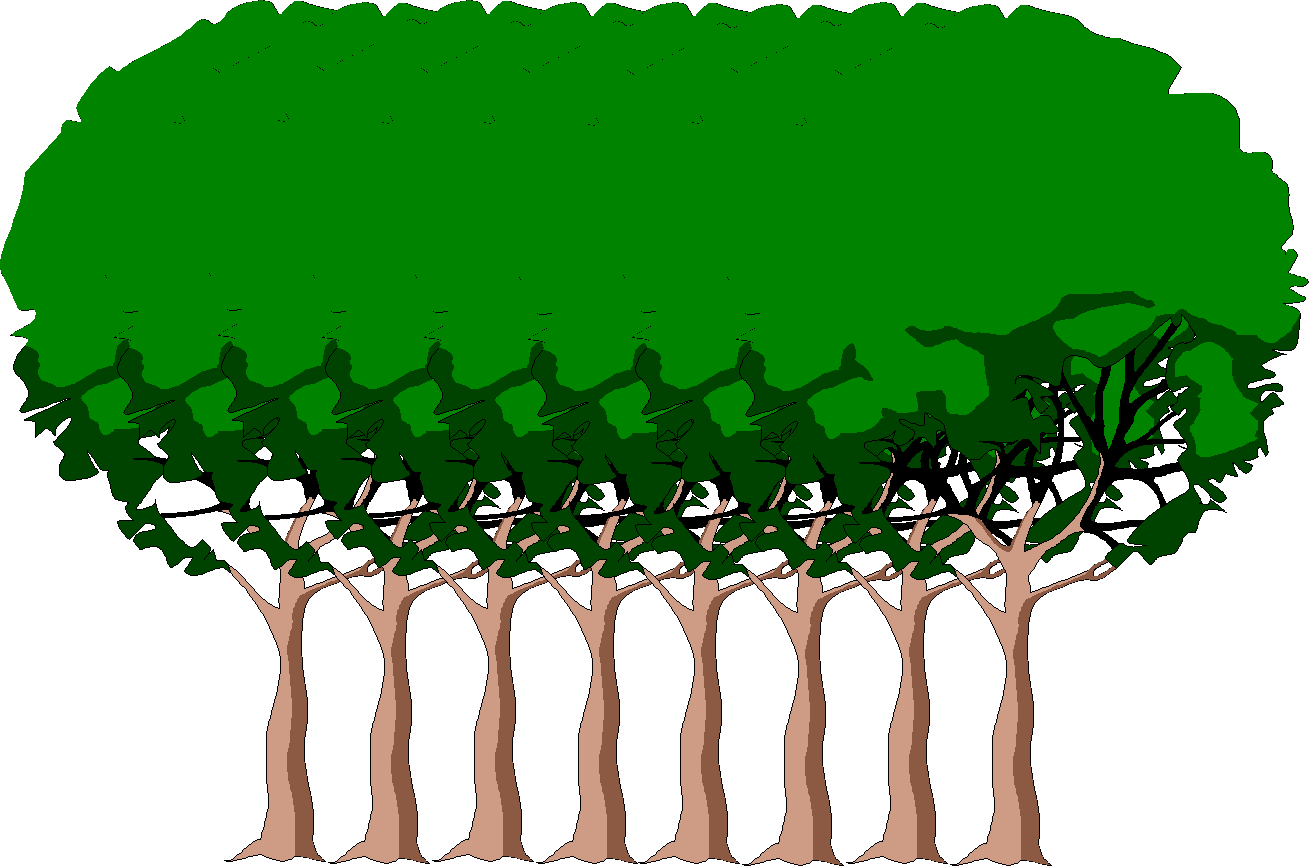
\includegraphics[height=1cm]{arbrex8}}
\put(4,0){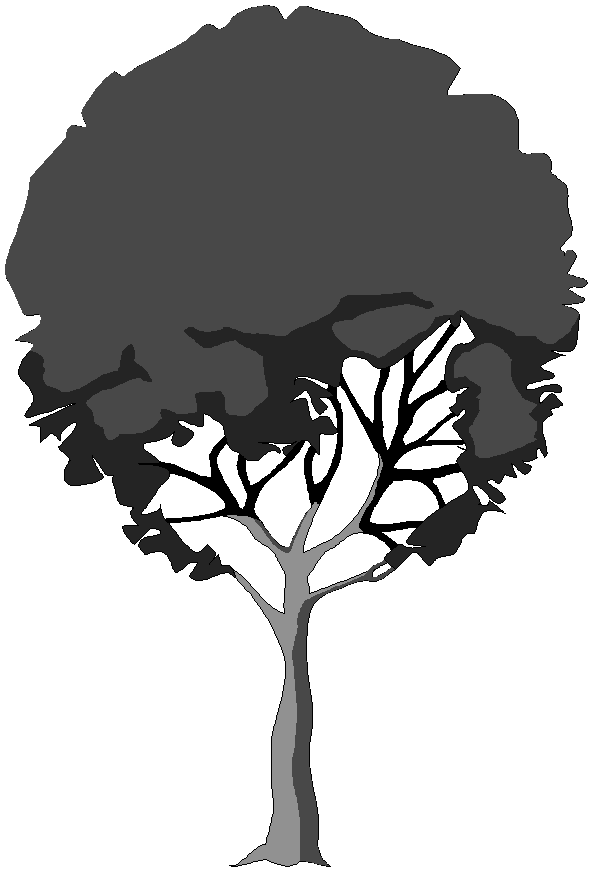
\includegraphics[height=2cm]{arbre}}
\put(8,0){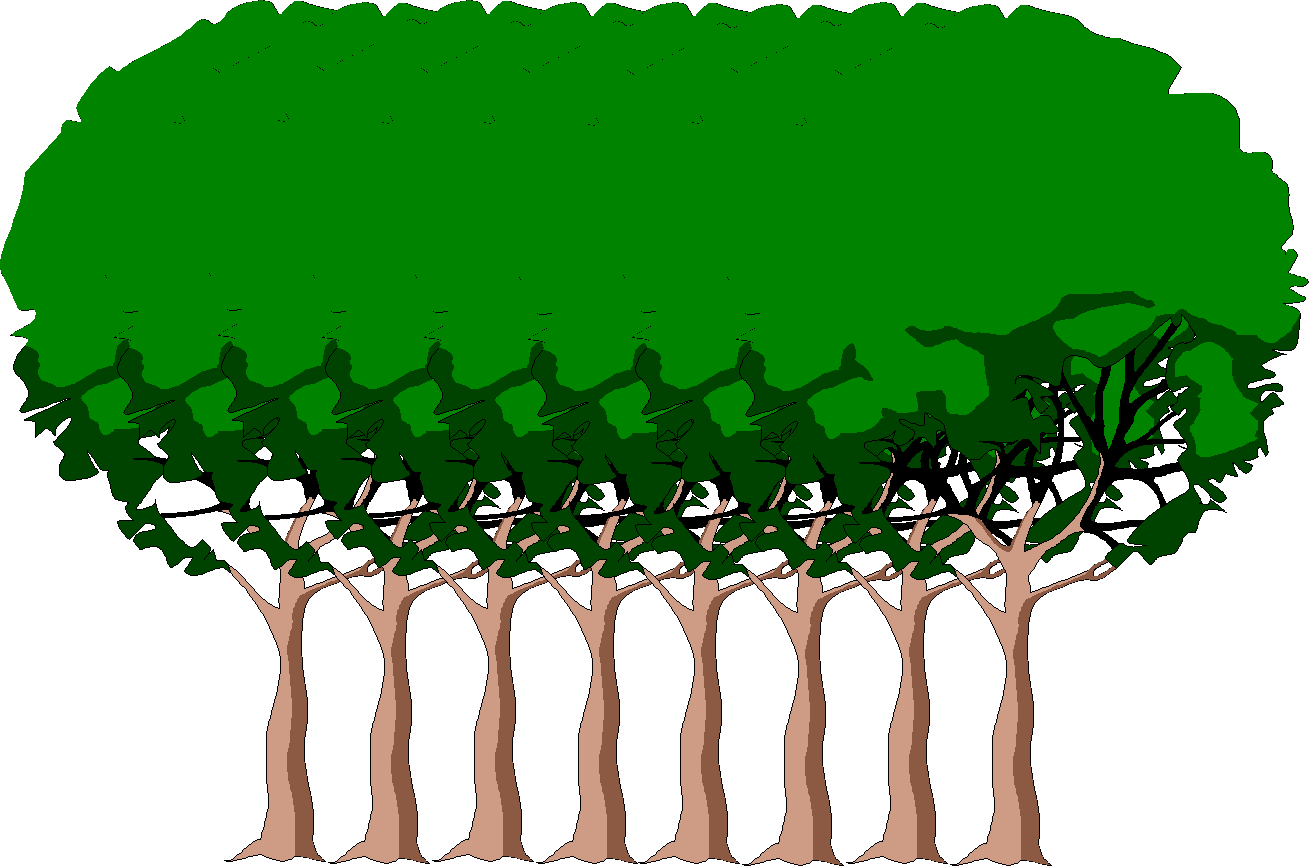
\includegraphics[height=3cm]{arbrex8}}
\put(0,-0.2){\vector(1,0){12}}\put(12.2,-0.25){Size ($D^2H$)}
\put(4.2,-0.6){$D^2H$}\put(-0.2,1.2){$n/2$ trees}
\put(9.3,3.2){$n/2$ trees}\put(4,2.2){Volume ?}
\multiput(0.3,-0.7)(4.4,0){2}{$\underbrace{\hspace{4.3cm}}_{\displaystyle\Delta}$}
\end{picture}
\end{center}
\caption[Sampling plan optimizing volume prediction precision for a particular tree]{Sampling plan optimizing volume prediction precision for a particular tree. The size deviation $\Delta$ must be as large as possible.\label{plan}}
\end{figure}
This sampling plan means that we can ignore the term dependent upon $D^{*2}H^*$ in (\ref{E1}), thus simplifying the relationship to:
\[
(1+E)^2-1\approx\frac{1}{n}
\]
For $E=5\,\%$, this gives us $n=10$ trees. Optimizing the sampling plan has therefore ``saved'' us measuring 88 trees compared to the plan that consisted in selecting trees at random. However, the optimized plan is restricted to estimating the volume of a $D^{*2}H^*$sized tree. It is not optimized for estimating the volume of other sized trees. This reasoning therefore clearly has its limitations as volume tables are not generally (or even never) constructed to predict the volume of only one size of tree.

Even more seriously, the optimized sampling plan is also reliant upon the super-population model and may yield erroneous estimations if it does not correspond to reality. This is illustrated in Figure \ref{bad}. The optimized sampling plan for a given $D^{*2}H^*$ size leads to the selection of extreme points (in black in Figure \ref{bad}) for the sample. This situation is critical for a linear regression as two groups of points far removed one from the other will give an elevated $R^2$ value without us really knowing what is happening between the two. If the linear relation assumed by the super-population model is correct (Figure \ref{bad} left), then there is no problem: the volume predicted by the tables (shown by a star) will indeed be close to the actual value (gray point). By contrast, if the super-population model is wrong, the predicted volume will be wrong: this is illustrated in Figure \ref{bad} on the right (where the sample points, in black, are exactly the same as those in Figure \ref{bad} on the left), where the size-volume relationship is in fact parabolic, not linear. In practice, the shape of the size-volume relationship (and therefore the volume tables) is not known in advance, and it is therefore best to sample trees across the entire size variation interval so as to visualize the nature of the size-volume relationship.

\begin{figure}[htb]
\begin{center}
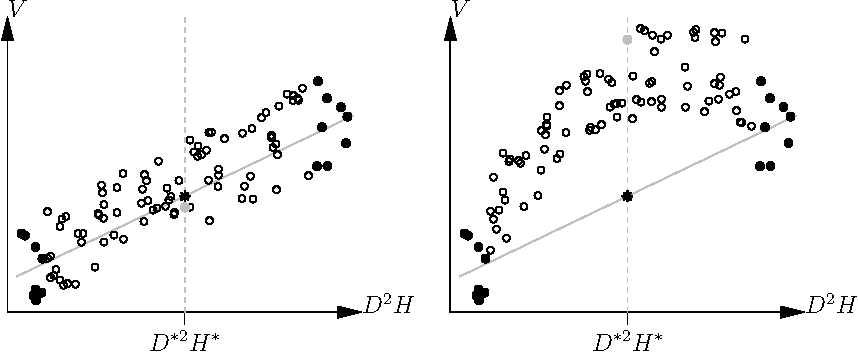
\includegraphics{badplan}
\end{center}
\caption[Volume prediction based on a linear regression constructed using extreme points when the size-volume relationship is indeed linear and when it is not]{Volume prediction based on a linear regression constructed using extreme points (in black) when the size-volume relationship is indeed linear (left) and when it is not (right). The black points are the same in both cases. The star indicates the volume predicted by the linear regression constructed using the black points while the gray points indicate the real volume corresponding to $D^{*2}H^*$.\label{bad}}
\end{figure}

\subsection{Predicting the volume of a stand\label{peup}}

Let us now assume that the goal is to predict the volume of an entire stand. Here, we must first assume that we measure dbh $D$ and height $H$ in \emph{all} the trees in the stand. Let $N$ be the number of trees in the stand (including the $n$ trees in the sample). Modulo renumbering of the trees therefore gives us a measurement of tree volume $V$ for $i=1$, \ldots, $n$ and a measurement of tree size $D^2H$ for $i=1$, \ldots, $N$. The estimator for the total volume of the stand deduced from the volume tables is therefore:
\[
V_{\mbox{\scriptsize tot}}=\sum_{i=1}^N(a+bD_i^2H_i)
\]
which may also be written: $V_{\mbox{\scriptsize
tot}}=N\bar{V}$, where $\bar{V}=a+b\overline{D^2H}$ is the mean volume of the trees in the stand, and $\overline{D^2H}=(\sum_{i=1}^ND_i^2H_i)/N$ is the mean dbh of the trees in the stand. To the extent that the volume tables are obtained by linear regression of ($V_1$, \ldots, $V_n$) against ($D_1^2H_1$, \ldots, $D_n^2H_n$), the numerical values of the coefficients $a$ and $b$ varify \citep[p.363]{saporta90}:
$\bar{V}_e=a+b\overline{D^2H}_e$, where
$\bar{V}_e=(\sum_{i=1}^nV_i)/n$ is the mean volume of the trees in the sample and $\overline{D^2H}_e=(\sum_{i=1}^nD_i^2H_i)/n$ is the mean size of the trees in the sample. By subtracting, we arrive at the following result:
\begin{equation}
\bar{V}=\bar{V}_e+b(\overline{D^2H}-\overline{D^2H}_e)\label{est}
\end{equation}
In this equation it is important to note that $\bar{V}$ and
$\overline{D^2H}$ are mean values for the entire stand while, $\bar{V}_e$ and $\overline{D^2H}_e$ are mean values for the sample. In addition $\overline{D^2H}$, $\overline{D^2H}_e$
and $\bar{V}_e$ are derived from actual measurement, while $\bar{V}$ is the quantity we are looking to estimate.

If we look at equation (\ref{est}), we recognize it as being a type of estimator that is widely used in sampling theory: the \emph{regression estimators}. The theoretical basis of regression estimators is described in detail in \citet[chapitre 7]{cochran77} and in \citet[chapitre 8]{thompson92}. A description of regression estimators used in forestry is given in \citet{vries86} and in \citet[chapitre 6]{shiver96} (the first is more theoretical, the second more applied). The theory of regression estimators applies in the case of a linear relationship between the quantity to be predicted ($\bar{V}$ in the example above) and an auxiliary variable ($\overline{D^2H}$ in the example above). By contrast, this theory is less well developed in the case of non-linear relations or multiple regressions, even though such cases often arise in connection with volume tables.

The semi-amplitude of the confidence interval at $\alpha$ (typically 5\,\%) of $\bar{V}$ is
(\citealp[p.199]{cochran77}; \citealp[p.83]{thompson92}):
\begin{equation}
t_{n-2}\;\hat{\sigma}\,\sqrt{\frac{1}{n}-\frac{1}{N}+
\frac{(\overline{D^2H}-\overline{D^2H}_e)^2}{\sum_{i=1}^n(D_i^2H_i
-\overline{D^2H}_e)^2}}\label{icpop}
\end{equation}
It can be seen that the minimum of this amplitude is zero, that is reached when entire stand is included in the sample ($n=N$, that means that $\overline{D^2H}=\overline{D^2H}_e$).
As before, the optimal sampling plan is such that 
$\overline{D^2H}_e$ is the closest possible to
$\overline{D^2H}$, with a maximal empirical variance of $D^2H$ in the sample.

When deriving the regression estimator we assumed that size $D^2H$ is measured for \emph{all} the trees in the stand in order to arrive at an estimation of total volume $V_{\mbox{\scriptsize tot}}$. In practice, a more realistic measurements protocol is as follows: the size of the trees in a sample of size $n'<N$ is measured; both size and volume are measured in a subsample of $n<n'$ of this sample. The volume vs dbh regression (i.e. the volume tables) is constructed using subsample values; this is then used to estimate the volume of the sample then, by extrapolation, that of the entire stand. This sampling strategy is called 
\emph{double sampling}. Its theory is described in \citet[section 12.6]{cochran77} and, more pragmatically, in \citet[chapitre 7]{shiver96}. Its use for estimating stand biomass was developed by \citet{cunia87c,cunia87,cunia87d}.

Finally, the properties of the regression estimator (\ref{est}) are well known in conventional sampling theory which does not require the hypothesis of a linear model (\ref{MLex}) but considers that the only source of variability is the sampling. In the case of a simple random sampling plan and a sufficiently large sample size $n$, the variance of $\bar{V}$ in conventional theory is approximately (\citealp[p.195]{cochran77};
\citealp[p.181]{shiver96}):
\begin{equation}
\widehat{\mbox{Var}}(\bar{V})=\frac{1-n/N}{n(n-2)}\left\{
\sum_{i=1}^n(V_i-\bar{V}_e)^2-\frac{\left[\sum_{i=1}^n
(V_i-\bar{V}_e)(D_i^2H_i-\overline{D^2H}_e)\right]^2}{\sum_{i=1}^n
(D_i^2H_i-\overline{D^2H}_e)^2}\right\}\label{VV}
\end{equation}
and the semi-amplitude confidence interval at $\alpha$ (typiquement 5\,\%) of $\bar{V}$ is approximately (\citealp[p.80]{thompson92}; \citealp[p.185]{shiver96}):
\[
t_{n-2}\;\sqrt{\widehat{\mbox{Var}}(\bar{V})}
\]
This last expression is considered as being more robust than expression (\ref{icpop}) when the super-population model (\ref{MLex}) strays from reality \citep[p.84]{thompson92}.

In conclusion, this simple example shows both the advantages and limitations of sampling for the construction of volume tables: advantages because sampling theory provides us with the minimum number of trees that need to be measured to reach a given precision in our predictions, and thereby optimize the sampling plan; limitations because this reasoning assumes that the form of the volume tables (and that the underlying super-population model) is known in advance and that the tables will be used for a given application. Neither of these prerequisites is met in practice. Also, the calculations that are relatively simple in the case of the linear model we have just described rapidly become hopelessly complex for more realistic models.

\section{Sampling to construct volume tables}

As a first step, let us consider the problem of predicting the volume or biomass of a particular tree using volume or biomass tables. How many trees need to be measured to construct the tables (\S\,\ref{size})? Which trees in the stand should be selected for measurement? This second question begs another: how should we sort the trees in the sample in relation to volume table entry variables, starting with the tree size (\S\,\ref{vent})? How, if necessary, should we stratify the sample (\S\,\ref{stratif})? Is it best to select individuals far apart in the forest, or on the contrary inventory all the trees in a given plot (\S\,\ref{sel})?

\subsection{Number of trees\label{size}}

Given the limitations of the sampling theory, the number of measured trees for volume or biomass (in other terms, the sample size) is generally selected empirically, based on rules established by experience. A general principle is that, for any given precision, the more variable the material, the larger the sample size: smaller sample sizes are required for a plantation of clones than for a natural tropical forest, for a given species than for a group of species, for a 10 ha plot than for a natural area. In certain cases, such as for root biomass, it is the cost of the measurements that determines the sample size rather than the desired precision of the predictions: the number of trees selected corresponds to an acceptable amount of work to obtain the measurements. As a rough guide, when constructing volume tables, the M�mento du forestier \citep[p.256]{ctft89} recommends measuring about 100 trees ``for one or more stands of recent plantation over a small surface area (e.g. silviculture research plots)''. \citet[p.108]{parde88} recommended the sample sizes given in Table \ref{eff}, that depend on the surface area of the zone in which the volume tables are to be used. Different volume and biomass tables have been compiled by \citet{zianis05} for Europe and by \citet{henry11} for sub-Saharan Africa. The sample sizes reported for the volume and biomass tables listed in these literature reviews give some idea of the sampling effort required. \citet{chave04} showed that when 300 trees were used to construct a biomass table, the resulting biomass estimation for a wet tropical stand (Barro Colorado Island in Panama) had a coefficient of variation of barely \decimal{3}{1}\,\%. This coefficient of variation rose above 10\,\% when the number of trees used to construct the biomass table fell below 50, with the coefficient of variation increasing approximately in proportion to $1/\sqrt{n}$ \citep[Figure 3]{chave04}. \Citet{vanbreugel11} noted the same type of decrease in estimation precision with the sample size used to construct the biomass table, for $n$ between 49 and 195 trees.

\begin{table}[htb]
\caption[Number of trees to be measured to establish a volume table for different surface areas over which the tables are to be used]{Number of trees to be measured to establish a volume table for different surface areas over which the tables are to be used: recommendations by \citet{parde88}.\label{eff}}
\begin{center}
\begin{tabular}{|lc|}
\hline Area & $n$
\\\hline Single, homogeneous stand & 30
\\ 15-ha plot & 100
\\ 1000-ha forest & 400
\\ Natural area & 800
\\ Species area & 2000 to 3000
\\\hline
\end{tabular}
\end{center}
\end{table}

The costlier an observation, in terms of measurement time and effort, the more the sampling plan tends to be determined by the sampling effort that workers are willing to make rather than by the desired precision of the estimation. As the above-ground biomass of a tree is more difficult to measure than the volume of its stem, biomass tables tend to be constructed using fewer observations than volume tables. Certain biomass tables are constructed from measurements in only a few trees (8 trees for \citealp{brown95} in Brazil, 12 trees for \citealp{ebuy11} in the Democratic Republic of Congo, 14 trees for \citealp{deans96}, 15 trees for \citealp{russell83} in Brazil).
Root tables, that require an even greater measurement effort, are often based on even smaller sample sizes. Tables constructed using such small samples are generally unreliable, and in any case are valid only very locally. However, these small datasets can subsequently be grouped together into more impressive datasets that have advantages for model fitting (on condition that the variability induced by the merging of these datasets can be controlled by effect covariables: age, wood density, etc. or by stratification factors: species, type of vegetal formation\ldots).

\subsection{Sorting trees\label{vent}}

The sorting of trees in the sample on the basis of their size (and more generally on the basis of table entry variables) can in principle be optimized. For example, in the case of a linear regression, the semi-amplitude of the confidence interval at $\alpha$ of the regression slope is \citep[p.367]{saporta90}:
\[
t_{n-2}\,\frac{\hat{\sigma}}{S_X\sqrt{n}}
\]
where $t_{n-2}$ is the quantile $1-\alpha/2$ of a Student's distribution with $n-2$ degrees of freedom, $\hat{\sigma}$ is the empirical standard deviation of the model's residuals, $n$ is sample size and $S_X$ is the empirical standard deviation of the entry variable $X$ in the sample:
\[
S_X^2=\frac{1}{n}\sum_{i=1}^n(X_i-\bar{X})^2\quad\mbox{where}\quad
\bar{X}=\frac{1}{n}\sum_{i=1}^nX_i
\]
Therefore, the higher the value of $S_X$ the more precise the estimation of the slope, which, for a set sample size, brings us back to a trees breakdown similar to that shown in Figure \ref{plan}. We have already seen the limitations of this reasoning: although the sampling plan that consists in selecting trees at the two extremities of the size gradient is optimal when the conditions of a linear relationship are met, it results in erroneous estimations when the relationship is not linear (Figure \ref{bad}). It is therefore preferable, in practice, to sample trees right across the size gradient in order to check the form of the relationship between their volume (or their mass) and their size.

The theory of response surfaces \citep{box87,goupy99,myers02}
can be used to optimize tree sorting on the basis of dbh (and more generally on the basis of table entry variables). We will not enter into the details of this theory here, but will simply sketch a few general principles. The first principle is to spread the tree size gradient of the sample as broadly as possible.

If the volume (or mass) variance is constant for all tree sizes, the rule is to measure the same number of trees in each size category (\citealp[p.108]{parde88};
\citealp[p.256]{ctft89}). It would be a mistake to form a sample by selecting in each size class a number of trees proportional to the magnitude of that class in the stand (in other words select the trees at random). But volume variance is rarely constant; generally it increases with tree size (heteroscedasticity of the residuals). The rule is therefore to increase sampling intensity in the most variable classes, thereby improving precision. In theory, the ideal approach is to measure a number of trees in a given size class proportional to the standard deviation of the tree volume in this class \citep[p.256]{ctft89}. In practice, when the entry variable is dbh, an empirical rule consists in selecting the same number of trees per basal area growth class and thus better represent large diameter trees \citep[p.256--257]{ctft89}.

This reasoning may be extended to other effect variables. If the table entry variable is $D^2H$, the trees may be sorted by $D^2H$. For multi-specific biomass tables, wood density $\rho$ is often used as the entry variable (with the specificity that it concerns the species not the tree). For multi-specific tables using diameter $D$ and specific wood density $\rho$ as entry variable, adequate sorting of the trees in the sample consists in dividing them evenly by dbh class and wood density class.

\subsection{Stratification\label{stratif}}

We have already seen for the sorting of trees into size classes that selecting trees at random, and thereby giving all trees and equal \emph{inclusion probability} is a suboptimal sampling plan. Stratification aims to take account of exogenous information to establish homogeneous sampling \emph{strata} and thus improve the precision of our estimations. The principle, in the same manner as previously, is to increase the sampling intensity of the most variable strata (relative to the other strata). Again using the example given in section \ref{simple}, the variance of the regression estimator $\bar{V}$ in the case of a stratified sampling approach becomes \citep[p.202]{cochran77}:
\begin{eqnarray}
\widehat{\mbox{Var}}(\bar{V}) &=&
\sum_h\left(\frac{N_h}{N}\right)^2
\frac{1-n_h/N_h}{n_h(n_h-2)}\left\{
\sum_{i=1}^{n_h}(V_{hi}-\bar{V}_{eh})^2\right.\nonumber
\\ && \left.-\frac{\left[\sum_{i=1}^{n_h}
(V_{hi}-\bar{V}_{eh})(D_{hi}^2H_{hi}-\overline{D^2H}_{eh})\right]^2}
{\sum_{i=1}^{n_h} (D_{hi}^2H_{hi}-
\overline{D^2H}_{eh})^2}\right\}\label{VVh}
\end{eqnarray}
where $h$ is the stratum, $N_h$ the number of individuals in the stand that belong to stratum $h$, $n_h$ is the number of individuals in the sample that belong to stratum $h$, $V_{ih}$
is the volume of the $i$th individual in stratum $h$ in the sample, $\bar{V}_{eh}$ is the empirical mean volume in stratum $h$ of the sample, etc.
This formula replaces (\ref{VV}). Let us now illustrate the precision gained by the stratification using a simple numerical example. Let us suppose, to simplify, that we have two strata, each corresponding to 50\,\% of the stand (such that $N_1/N=N_2/N=\decimal{0}{5}$), and that the sampling in each stratum is such that the second term between brackets in (\ref{VVh}) is negligible. Let us also assume that $n_1\ll N_1$ and $n_2\ll N_2$. The variance of the regression estimator in this case is approximately proportional to:
\[
\widehat{\mbox{Var}}(\bar{V})\propto \frac{1}{n_1-2}\left\{
\frac{1}{n_1}\sum_{i=1}^{n_1}(V_{1i}-\bar{V}_{e1})^2\right\}
+\frac{1}{n_2-2}\left\{\frac{1}{n_2}\sum_{i=1}^{n_2}(V_{2i}
-\bar{V}_{e2})^2\right\}
\]
The terms in brackets represent within-strata variances in volume. Let us suppose that the standard deviation of the volume is 4 m$^3$ in the first stratum and 2 m$^3$ in the second. Total sample size is set at $n_1+n_2=60$ individuals.
If we take account of the stratification, i.e. if we select the number of trees in each stratum in proportion to the frequency $N_h/N$ of the stratum in the stand, then in this case we have the same number of trees in each stratum of the sample: $n_1=n_2=30$ individuals. The variance of the regression estimator is therefore approximately:
\[
\frac{4^2}{30-2}+\frac{2^2}{30-2}=\decimal{0}{71}\mbox{ m}^6
\]
By contrast, if we set the number of trees in each stratum in proportion to the standard deviation of the volume in the stratum, then: $n_1=2n_2$, giving $n_1=40$ individuals and $n_2=20$ individuals. The variance of the regression estimator is therefore approximately:
\[
\frac{4^2}{40-2}+\frac{2^2}{20-2}=\decimal{0}{64}\mbox{ m}^6
\]
It can thus be seen that from the standpoint of estimator variance, $30+30$ does not equal $40+20$. We can also check that the minimum of the function that at $n_1$ associates
$16/(n_1-2)+4/(58-n_1)$ is obtained for $n_1=\decimal{39}{333}$.

From the standpoint of sampling theory, stratification aims to increase the precision of the estimation by fitting the sampling plan to the variability in each stratum. But from the standpoint of constructing volume tables, stratification has a second aim that is just as important as the first: check that the relationship between tree volume (or biomass) and size is the same in each stratum and, if needed, break down the tables into as many relations as necessary. This second point is implicit in equation (\ref{VVh}) that is based on the fitting of a different slope $b$ (see equation \ref{reg}) in each stratum.

In short, stratification aims to explore the variability of the study area to (\textit{i}) if necessary vary the form of the tables in accordance with the strata, and
(\textit{ii}) fit the sampling plan to the variability in the strata. Often when constructing volume tables, point (\textit{i}) is predominant over point (\textit{ii}), whereas the reverse is true in sampling theory. Figure \ref{mel} illustrated these two aims.

\begin{figure}[p]
\begin{center}
\includegraphics{badmel}
\end{center}
\caption[Predicting volume from tree size in two strata]{Predicting volume from tree size in two strata (black and white points): top left: the two strata corresponding to the two variances of the residuals (higher variance for the white than the black points) but the relationship is the same; top right: both the variance and the relation are different in the two strata; bottom: the situation is the same as top right but the second stratum has been subsampled such that we are led to believe that we are dealing with the same relation in the two strata.\label{mel}}
\end{figure}

\subsubsection{Stratification factors}

Any factor that can explain the variability in the study area may be envisaged: stand age (above all for plantations), fertility, station, silvicultural treatments, variety or species, altitude, depth of the water table, etc. (\citealp[p.106]{parde88}; \citealp[p.255]{ctft89}). Stratification factors may be nested: stratification according to morpho-pedological region, then according to fertility in each region, then according to age in each fertility class, then according to density in each age class. The ``finenesse'' of the stratification factors must also be adapted to match the context. The stratification factors employed are not the same when reasoning on a global scale like \citet{brown97}, on a landscape scale like \citet{vanbreugel11}, or on the scale of a plantation of clones like \citet{saintandre05}. \citet{brown97} proposes ``all-species'' tables for climatic areas (dry forests, wet forests). At the other extreme, on an ``eddy-correlation'' plot, and with the aim of comparing NEP estimations, trees may be stratified according to plot age, season and flux tower ``foot-print''.

\subsubsection{Species as stratification factor}

When dealing with natural formations that contain several species, the species may also be considered as stratification factor. Here, it is routine practice to construct volume tables separately for each species (or at least the most abundant species), then attempt to group gender or group together all the species (``all species'' table). By merging the datasets we increase sample size which can be advantageous if this compensates for the increase in variability resulting from the mix of different species. In comparison with a mono-specific model, a multi-specific model introduces a prediction bias that may be viewed as between-species variability. As an illustration, \Citet{vanbreugel11} quantified the prediction bias resulting from the aggregation of several species. Therefore, merging the data from several species is advantageous if the gain in within-species variability provided by this merger compensates for the between-species variability introduced. However, a check must be made that (\textit{i}) this merger is meaningful and that (\textit{ii}) the sample sizes for the different species are comparable (Figure \ref{mel}). If from the outset we are looking to construct ``all species'' volume table (which is often the case for natural stands), care must be taken to ensure that the individuals are selected for the sample independently of their species, such that the tables are not biased in favor of one particular species.

\subsubsection{Allocating to strata}

Once the strata have been identified, the sampling plan must be adapted to it following empirical rules. If we have an {\it a priori} estimation of volume variability (for volume tables) or biomass variability (for biomass tables) for each stratum, the empirical rule is to select a sampling intensity in proportion to the standard deviation in each stratum. If no {\it a priori} estimation of the variability is available, then a constant sampling intensity should be used in each stratum (this does not correspond to random sampling if the strata do not have the same frequency in the stand).

\subsubsection{Parameterized models}

Strata-related information is then incorporated into the volume model by establishing different models for each stratum. We can then test whether the models for the two strata are significantly different and, if appropriate, merge the two datasets to construct a single model. We could also construct a parameterized model from several models for different strata by following the principle of the mixed model: the model's parameters themselves become functions of the variables defining the strata. These different points will be developed in the sections below, devoted to the actual construction of volume/biomass models. By way of an example, \citet{ketterings01} developed individual, single-entry biomass models of the power form:
\[
B=aD^b
\]
where $D$ is the dbh and $B$ biomass of different trees of different species at different sites in the Jambi province of Sumatra in Indonesia. The site factor was then taken into account in parameter $b$ that was written $b=2+c$, where $c$ is the parameter in the allometric equation that links height to dbh at each site: $H=kD^c$. The species factor was taken into account in parameter $a$ that was written $a=r\rho$, where $\rho$ is the wood density of the species and $r$ is a constant parameter. The model finally obtained, and valid for all the species at all the sites, is a parameterized model:
\[
B=r\rho D^{2+c}
\]

\subsection{Selecting trees\label{sel}}

Once the composition of the sample has been established, the trees must be identified and measured in the field. Given that these measurements involve a great deal of work and, when involving biomass, are destructive, the trees used must be selected with great care. A strategy adopted by some when constructing biomass tables is to cut all the trees within a given area (for example half a hectare). This has the advantage of ``killing two birds with one stone'' in that it provides both a biomass estimate for the stand and individual observations for the construction of a model. From a practical standpoint, the space created by the cutting of the first trees facilitates the subsequent cutting of the next. But this strategy has a major drawback: as the tree size distribution of the trees in the stand has only a very small likelihood of coinciding with the desired sorting of the trees in the sample by size class, the tree size distribution in the sample is suboptimal. The same applies for any factor in the structure of the sample (wood density classes, strata, etc.). Also, the scale of this disturbance in the stand may have unexpected consequences. For instance, \citet{djomo10} reported on a plot that was invaded by ants after the trees had been felled, to such an extent that it was impossible to make any tree biomass measurements. This tree selection strategy should therefore be avoided in areas infested by \textit{Wasmannia} ants as their attacks are highly dangerous.

Rather than selecting all the trees within a given area, preference should be given to selecting stems one by one depending on the requirements of sample constitution. This strategy may be longer to implement as it requires the identification of individual trees. In view of the difficulties inherent to measuring tree biomass (see chapter \ref{ter}), preference should be given to trees that match the criteria of the sampling plan and are most easily accessible.

\section{Sampling for stand estimations\label{sampeup}}

Let us now consider the problem of predicting the volume or biomass of a stand. In a rigorously statistical manner, we need to consider the entire error propagation chain as described in Figure \ref{cha} \citep{parresol99}. This raises questions of double sampling and regression estimator, as described in section \ref{peup}. \citet{cunia87c,cunia87,cunia87d}, \citet{chave04} and \citet{vanbreugel11} are rare examples where the entire error propagation chain was indeed taken into account, and where the biomass estimation error for a stand was related to the sample size used to construct the biomass table necessary for this estimation. In practice the problem is generally simplified by considering the table as exact and not suffering from any prediction error. This approximation --- which disconnects the sampling of the stand used to predict its volume or biomass, from the sampling of the trees used to construct the model --- reduces the sampling to a conventional forest inventory problem.

We will not dwell here on this question of forest inventory, first because it is not central to this guide's purpose, and second because entire books have already been devoted to the subject \citep{loetsch73,lanly81,vries86,schreuder93,shiver96,west09}. We will nevertheless describe a few developments relating to the estimation of stand biomass.

\subsection{Sampling unit}

Whereas it is entirely suitable, when constructing a biomass model, to select trees for the sample in an individual manner, this sampling strategy is unrealistic when estimating the biomass of a stand.
We should rather in this case opt for a strategy consisting in measuring all the trees within a given area, and if necessary repeating this approach on another area to increase sample size. This area, or plot, thus becomes the sampling unit. Let $n$ be the number of plots inventoried, $N_i$ be the number of trees found in the $i$th plot ($i=1$, \ldots, $n$), and $B_{ij}$ be the biomass of the $j$th tree in the $i$th plot ($j=1$, \ldots, $N_i$), calculated using the biomass model and the measured characteristics of the tree. The number $N_i$ is random, but for a given tree the prediction of $B_{ij}$ is considered as deterministic. The biomass of the $i$th plot is therefore: $B_i=\sum_{j=1}^{N_i}B_{ij}$.

Let $A$ be the area of a sampling plot and $\mathcal{A}$ be the area of the stand. In the super-population model the biomass of the stand is therefore estimated by: $(\mathcal{A}/A)\,\bar{B}$, where $\bar{B}=(\sum_{i=1}^nB_i)/n$ is the mean biomass of a plot. It is generally considered that $A$ and $\mathcal{A}$ are accurately known parameters. The stand biomass estimation error therefore stems from that of mean biomass $\bar{B}$.

\subsection{Relation between coefficient of variation and plot size}

According to the central limit theorem, the confidence interval at the threshold $\alpha$ for the expectation of plot biomass is approximately (this expression is accurate when the biomass follows a normal distribution, or when the number of plots approaches infinity) \citep[p.304]{saporta90}:
\[
\bar{B}\pm t_{n-1}\frac{S_B}{\sqrt{n-1}}
\]
where $t_{n-1}$ is the quantile $1-\alpha/2$ of a Student distribution with $n-1$ degrees of freedom, and $S_B$ is the empirical standard deviation of plot biomass:
\[
S_B^2=\frac{1}{n-1}\sum_{i=1}^n(B_i-\bar{B})^2
\]
By definition, the precision of the estimation $E$ at the threshold $\alpha$
is the ratio of the semi-amplitude of the confidence interval at the threshold $\alpha$ to the mean biomass:
\begin{equation}
E=t_{n-1}\frac{S_B}{\bar{B}\sqrt{n-1}}=t_{n-1}\frac{\mathrm{CV}_B}{\sqrt{n-1}}
\label{E}
\end{equation}
where $\mathrm{CV}_B=S_B/\bar{B}$ is the biomass coefficient of variation. By rounding $t_{n-1}$ to 2, the sample size $n$ required to reach a given estimation precision $E$ is therefore:
\[
n\simeq\bigg(\frac{2\mathrm{CV}_B}{E}\bigg)^2+1
\]
The biomass coefficient of variation for a plot of area $A$ is therefore the essential factor when constructing the sampling plan. Also, as area $A$ of the plots is not in principle known, the relation between the biomass coefficient of variation and the area $A$ of the plots must in fact be determined.

The exact derivation of this relation between $A$ and $\mathrm{CV}_B$
needs a model capable of describing the spatial distribution of the trees. The theory of point processes meets this need \citep{cressie93,stoyan94}. It is feasible, in a point process, to calculate exactly the relationship between $A$ and $\mathrm{CV}_B$ but this is rather complex \citep{picard04d,picard07d}. The exact calculation brings two things to our notice:
\begin{enumerate}
\item although plot \emph{shape} has an effect on the coefficient of variation (as already demonstrated empirically, see \citealp{johnson52,bormann53}), it has a negligible effect compared to plot size;
\item the relation between $A$ and $\mathrm{CV}_B$ can be approached by a power relation \citep{fairfield38,picard11b}:
\[
\mathrm{CV}_B=kA^{-c}
\]
\end{enumerate}
In practice it is this power relation that is most often specified. Intuitively, the value $c=\decimal{0}{5}$
corresponds to a random spatial biomass distribution within the stand; a value of $0<c<\decimal{0}{5}$ corresponds to an clustered spatial biomass distribution; and a value $c>\decimal{0}{5}$ corresponds to a regular spatial biomass distribution \citep[p.284]{ctft89}. Using biomass data for a large plot in Paracou, French Guiana, \citet{wagner10} found:
\[
\mathrm{CV}_B=557\times A^{-0.430}\qquad\mbox{($A$ in m$^2$,
CV$_B$ in \%)}
\]
If compared to the above definition, this corresponds to a slightly aggregated spatial biomass distribution. In the Brazilian Amazon, \citet{keller01} found the following relationship (fitted to the data in their Figure 4 with
$R^2=\decimal{0}{993}$ on log-transformed data):
\[
\mathrm{CV}_B=706\times A^{-0.350}\qquad\mbox{($A$ in m$^2$,
CV$_B$ in \%)}
\]
The lowest (absolute) value for the exponent is indicative of a more aggregated distribution than in French Guiana. A similar study was conducted by \citet{chave03}
using data from a 50 ha plot on Barro Colorado Island, Panama. \citet{chave03} in their Table 5 reported 95\,\%
interval amplitude values not for the biomass expectation of a plot, but for biomass expectation by unit area. The amplitude of the 95\,\% confidence interval for the biomass expectation of a plot therefore corresponds to the amplitude reported by \citet{chave03} times plot area, i.e.:
\[
2t_{n-1}\frac{S_B}{\sqrt{n-1}}=\Delta\times A
\]
where $\Delta$ is the amplitude of the 95\,\% confidence interval reported by \citet{chave03} in their Table 5. We can deduce from this:
\[
\mathrm{CV}_B=\frac{S_B}{\bar{B}}=\frac{\Delta
A\sqrt{n-1}}{2t_{n-1}\bar{B}}=\frac{\Delta
\sqrt{n-1}}{2t_{n-1}\mu}
\]
where $\mu$ is mean biomass per unit area, and reported as 274~Mg\,ha$^{-1}$ in the study by \citet{chave03}. Table
\ref{c03} supplements Table 5 by \citet{chave03} with the calculated value of $\mathrm{CV}_B$. The $\mathrm{CV}_B$
values given in Table \ref{c03} closely fit ($R^2=\decimal{0}{998}$ on log-transformed data) the following power relation with plot size:
\[
\mathrm{CV}_B=942\times A^{-0,450}\qquad\mbox{($A$ in m$^2$,
CV$_B$ in \%)}
\]
Biomass variability (expressed by the value of the multiplier $k=942$) was greater than at Paracou, but the spatial structure of the biomass (expressed by the exponent $c=\decimal{0}{45}$) fairly similar to that observed in Paracou by \citet{wagner10}. Also, the fact that $c$ approached \decimal{0}{5} showed that the biomass was only slightly spatially aggregated. \citet{chave03} underlined that there was no significant spatial autocorrelation of the biomass (which would correspond to $c=\decimal{0}{5}$, or to a constant value of $\Delta$).

\begin{table}
\caption[Coefficient of variation in relation to plot size]{Coefficient of variation in relation to plot size: data drawn from Table 5 by \citet{chave03} for Barro Colorado Island, Panama.\label{c03}}
\begin{center}
\begin{tabular}{|rrrr|}\hline
$A$     & $n$  & $\Delta$        & $\mathrm{CV}_B$\\ %
(m$^2$) &      & (Mg\,ha$^{-1}$) & (\%) \\\hline%
100     & 5000 & \decimal{17}{4} & \decimal{114}{5}\\ %
200     & 2500 & \decimal{18}{7} & \decimal{87}{0} \\ %
400     & 1250 & \decimal{20}{0} & \decimal{65}{7} \\ %
1000    & 500  & \decimal{21}{4} & \decimal{44}{4} \\ %
2500    & 200  & \decimal{20}{1} & \decimal{26}{2} \\ %
5000    & 100  & \decimal{22}{4} & \decimal{20}{5} \\ %
10000   &  50  & \decimal{23}{5} & \decimal{14}{9} \\ %
\hline
\end{tabular}
\end{center}
\end{table}

\subsection{Selecting plot size}

The size of sampling plots may be selected in such a way to optimize the precision of the estimation for a given sampling effort \citep{bormann53,schreuder87,hebert88}, or in a manner to minimize sampling effort for a given estimation precision \citep{zeide80,gambill85,cunia87,cunia87d}.
These two points of view are dual one to the other and lead to the same optimum. The sampling effort may be quantified simply by the sampling rate $n\times A/\mathcal{A}$ or, more realistically, by a cost whose expression is more complex. Let us examine these two options.

\subsubsection{Fixed sampling rate}

At a constant sampling rate, the area $A$ and the number $n$ of sampling plots are linked by an inversely proportional relation: $n\propto1/A$. Choosing appropriate plot size boils down to the following question: ``is it better to select a few large plots or many small plots?'', also called the SLOSS compromise (for ``single large or several small'';
\citealp{lahti85}). If we calculate the relation $n\propto1/A$ in (\ref{E}) (and considering that $t_{n-1}/\sqrt{n-1}$ is little different from $2/\sqrt{n}$):
\[
E\propto2\;\mathrm{CV}_B\;\sqrt{A}
\]
If the spatial distribution of the biomass is random, $\mathrm{CV}_B\propto A^{-0,5}$ and therefore the precision of the estimation $E$ is independent of the area $A$ of the plots. If the spatial distribution of the biomass is aggregated, $\mathrm{CV}_B\propto A^{-c}$ with $c<\decimal{0}{5}$ and therefore $E\propto A^{0,5-c}$ with $\decimal{0}{5}-c>0$: then the smaller the plot area $A$, the greater the precision of the estimation (low value of $E$). In this case, and with a fixed sampling rate, it is therefore better to select several small plots than a few large plots. This is demonstrated by Table \ref{c03}, where we can see that the value of $\Delta$ decreases when $A$ decreases (this decrease is only slight as $c$ is close to \decimal{0}{5}). If the spatial distribution of the biomass is regular, $\mathrm{CV}_B\propto A^{-c}$ with $c>\decimal{0}{5}$ and therefore $E\propto A^{0,5-c}$ with $\decimal{0}{5}-c<0$: the larger the plot area $A$ the better the precision of the estimation (low value of $E$). In this case, and with a fixed sampling rate, it is therefore better to select a few large plots than many small plots.

The parameters measured in biology in most cases have an aggregated spatial distribution ($c<\decimal{0}{5}$), sometimes random distribution ($c=\decimal{0}{5}$), and only rarely a regular distribution ($c>\decimal{0}{5}$) \citep{fairfield38}. In other words, the SLOSS compromise is in most cases resolved to the benefit of a multitude of small plots. If we push this reasoning to its limit, we see that the precision of the estimation would be optimal ($E$ minimal) for $A=0$, i.e. by selecting an infinite number of plots of zero size! This illustrates the limits of this reasoning. When we quantify the sampling effort by the sampling rate $nA/\mathcal{A}$, we assume implicitly that the sampling cost, i.e. the time or money necessary for the sampling, is proportional to $nA$. This means that we consider only an area-based cost, i.e. a sampling cost that is proportional to the inventoried area.

\subsubsection{Sampling cost}

In actual fact, the area-based cost is only one component of the sampling cost. Strictly speaking, the inventory made of the sampling plots, and whose duration is indeed proportional to the inventoried area, is not the only task that takes time. Staking out the boundaries of the sampling plots also takes time. And this time is proportional to the cumulated length of their boundaries: this is therefore a linear cost. Moving from one plot to another also takes time. It is therefore more realistic to measure sampling effort by a cost that includes all these tasks rather than simply by the sampling rate. If we measure this cost in terms of time, and if the sampling plots are square, the sampling cost would for example be \citep{zeide80,gambill85}:
\[
C=\alpha\;nA+\beta\times4n\sqrt{A}+\gamma\;d(n,A)
\]
where $\alpha$ is inventory time by unit area, $\beta$ is staking out time by unit length ($4\sqrt{A}$ corresponds to the boundaries of a square plot of area $A$), $\gamma$ is travel speed, and $d(n,A)$
is the length of the path linking the $n$ sampling plots. This sampling cost expression can be further supplemented to take account of other tasks. The reasoning followed in the previous section consisted of $\beta=\gamma=0$. If $\beta>0$ and $\gamma>0$, the solution to the SLOSS compromise is now no longer $A=0$ in the case of aggregated spatial biomass distribution ($c<\decimal{0}{5}$).

\subsubsection{Other constraints}

However, it would be too restrictive to limit the question of sampling the biomass of a stand to a question of estimation precision. Often, the question is not limited to estimating a stand's biomass since a number of goals are pursued simultaneously. For instance, we may also be interesting in determining biomass variations over time. Mortality processes must also be considered in this case, and the inventoried area may therefore be far larger \citep{chave03,chave04,rutishauser10,wagner10}. Or we may be looking to estimate plot biomass in order to determine a relation with satellite image indices and thereby extrapolate the biomass estimation to a landscape scale. In this case the area of the sampling plots is also constrained by the resolution of the satellite images and by the smallest area necessary to calculate satellite remote sensing indices.

Additionally, the type of sampling plan implicitly considered here, i.e. a simple random plan using plots of a fixed size, is rarely the most efficient (\textit{i.e.} with the best estimation precision for a given sampling cost). On the scale of a landscape consisting of different forest types, other sampling strategies may turn out to be more efficient \citep{whraton87,vanbreugel11}. Compared to a simple random plan with a single plot size, a stratified sampling plan will be more costly (as stratification comes at a cost) but would provide a more precise estimation. A cluster sampling plan is less costly (less traveling) but provides a less precise estimation. Specific forest inventory techniques such as distance sampling \citep{magnussen08,magnussen08b,picard07d,picard05} or using Bitterlich's relascope \citep{schreuder93,west09}, share the feature of being based on plots of variable sizes, and can also be more efficient alternatives to fixed-size plot approaches.
